\documentclass[smallextended]{svjour3}
\usepackage[]{graphicx}\usepackage[]{color}
% maxwidth is the original width if it is less than linewidth
% otherwise use linewidth (to make sure the graphics do not exceed the margin)
\makeatletter
\def\maxwidth{ %
  \ifdim\Gin@nat@width>\linewidth
    \linewidth
  \else
    \Gin@nat@width
  \fi
}
\makeatother

\definecolor{fgcolor}{rgb}{0.345, 0.345, 0.345}
\makeatletter
\@ifundefined{AddToHook}{}{\AddToHook{package/xcolor/after}{\definecolor{fgcolor}{rgb}{0.345, 0.345, 0.345}}}
\makeatother
\newcommand{\hlnum}[1]{\textcolor[rgb]{0.686,0.059,0.569}{#1}}%
\newcommand{\hlstr}[1]{\textcolor[rgb]{0.192,0.494,0.8}{#1}}%
\newcommand{\hlcom}[1]{\textcolor[rgb]{0.678,0.584,0.686}{\textit{#1}}}%
\newcommand{\hlopt}[1]{\textcolor[rgb]{0,0,0}{#1}}%
\newcommand{\hlstd}[1]{\textcolor[rgb]{0.345,0.345,0.345}{#1}}%
\newcommand{\hlkwa}[1]{\textcolor[rgb]{0.161,0.373,0.58}{\textbf{#1}}}%
\newcommand{\hlkwb}[1]{\textcolor[rgb]{0.69,0.353,0.396}{#1}}%
\newcommand{\hlkwc}[1]{\textcolor[rgb]{0.333,0.667,0.333}{#1}}%
\newcommand{\hlkwd}[1]{\textcolor[rgb]{0.737,0.353,0.396}{\textbf{#1}}}%
\let\hlipl\hlkwb

\usepackage{framed}
\makeatletter
\newenvironment{kframe}{%
 \def\at@end@of@kframe{}%
 \ifinner\ifhmode%
  \def\at@end@of@kframe{\end{minipage}}%
  \begin{minipage}{\columnwidth}%
 \fi\fi%
 \def\FrameCommand##1{\hskip\@totalleftmargin \hskip-\fboxsep
 \colorbox{shadecolor}{##1}\hskip-\fboxsep
     % There is no \\@totalrightmargin, so:
     \hskip-\linewidth \hskip-\@totalleftmargin \hskip\columnwidth}%
 \MakeFramed {\advance\hsize-\width
   \@totalleftmargin\z@ \linewidth\hsize
   \@setminipage}}%
 {\par\unskip\endMakeFramed%
 \at@end@of@kframe}
\makeatother

\definecolor{shadecolor}{rgb}{.97, .97, .97}
\definecolor{messagecolor}{rgb}{0, 0, 0}
\definecolor{warningcolor}{rgb}{1, 0, 1}
\definecolor{errorcolor}{rgb}{1, 0, 0}
\makeatletter
\@ifundefined{AddToHook}{}{\AddToHook{package/xcolor/after}{
\definecolor{shadecolor}{rgb}{.97, .97, .97}
\definecolor{messagecolor}{rgb}{0, 0, 0}
\definecolor{warningcolor}{rgb}{1, 0, 1}
\definecolor{errorcolor}{rgb}{1, 0, 0}
}}
\makeatother
\newenvironment{knitrout}{}{} % an empty environment to be redefined in TeX

\usepackage{alltt}
\newcommand{\SweaveOpts}[1]{}  % do not interfere with LaTeX
\newcommand{\SweaveInput}[1]{} % because they are not real TeX commands
\newcommand{\Sexpr}[1]{}       % will only be parsed by R

    
\smartqed  % flush right qed marks, e.g. at end of proof

\usepackage[colorlinks=true,linkcolor={blue},citecolor={blue},urlcolor={blue}]{hyperref}
%\usepackage{caption}
% Add longtable and ctable packages
\usepackage{longtable,ctable}
\usepackage{amsmath}
\usepackage{amssymb}
\usepackage{amsfonts}
\usepackage{multirow}
%\usepackage{amsthm}
\usepackage{graphicx}

\usepackage{booktabs}
%\usepackage{bookmark}

%\usepackage{caption}
%\usepackage{capt-of}

\usepackage{amsmath}
\usepackage{graphicx}
\usepackage{mathptmx}
\usepackage{natbib}

\usepackage{setspace}

%\usepackage{tikz-feynman}
%\usepackage{tikz} 
%\usetikzlibrary{positioning}
\usepackage[utf8]{inputenc}
\usepackage{pgf}


\usepackage{algorithm}
\usepackage{algpseudocode}
\usepackage{enumerate}

\usepackage{threeparttable}

\raggedbottom

\newcommand{\R}{R}
\newcommand{\gbsg}{gbsg}

%\def\FsNg{\hbox{FS}(M_{g})}

\def\FsNg{\hbox{FS-M}}

\def\hhat{\hat\theta(\hat{H})}
\def\hchat{\hat\theta(\hat{H}^{c})}
\def\hknow{\hat\theta(H)}
\def\hcknow{\hat\theta(H^{c})}
\def\hplim{\theta^{\dagger}(H)}
\def\hcplim{\theta^{\dagger}(H^{c})}

\def\sumin{\sum_{i=1}^n}
\def\nsumin{n^{-1}\sum_{i=1}^n}

\def\ns{n_{0}+n_{1}}
\def\na{n_{0}}
\def\nb{n_{1}}

\newcommand{\indep}{\perp \!\!\! \perp}

\textheight=9.25in \textwidth=6.0in 
\topmargin=0in
\evensidemargin=0in \oddsidemargin=0in



\begin{document}





\begin{knitrout}
\definecolor{shadecolor}{rgb}{0.969, 0.969, 0.969}\color{fgcolor}\begin{kframe}
\begin{alltt}
\hlcom{# Remove unnecessary packages (eg SPlit and Virtual Twins and psych)}
\hlcom{# requiredPackages <-}
\hlcom{# c('grf','policytree','data.table','randomForest','survival','SPlit','plyr',}
\hlcom{#'cubature','formatR','kableExtra','knitr','ggplot2','gridExtra','aVirtualTwins','psych')}

\hlstd{requiredPackages} \hlkwb{<-} \hlkwd{c}\hlstd{(}\hlstr{"grf"}\hlstd{,} \hlstr{"policytree"}\hlstd{,} \hlstr{"data.table"}\hlstd{,} \hlstr{"randomForest"}\hlstd{,} \hlstr{"survival"}\hlstd{,}
    \hlstr{"plyr"}\hlstd{,} \hlstr{"cubature"}\hlstd{,} \hlstr{"knitr"}\hlstd{)}

\hlstd{ipak} \hlkwb{<-} \hlkwa{function}\hlstd{(}\hlkwc{pkg}\hlstd{) \{}
    \hlstd{new.pkg} \hlkwb{<-} \hlstd{pkg[}\hlopt{!}\hlstd{(pkg} \hlopt{%in%} \hlkwd{installed.packages}\hlstd{()[,} \hlstr{"Package"}\hlstd{])]}
    \hlkwa{if} \hlstd{(}\hlkwd{length}\hlstd{(new.pkg)} \hlopt{>} \hlnum{0}\hlstd{) \{}
        \hlkwd{install.packages}\hlstd{(new.pkg,} \hlkwc{dependencies} \hlstd{=} \hlnum{TRUE}\hlstd{,} \hlkwc{quietly} \hlstd{=} \hlnum{TRUE}\hlstd{,} \hlkwc{verbose} \hlstd{=} \hlnum{FALSE}\hlstd{,}
            \hlkwc{logical.return} \hlstd{=} \hlnum{FALSE}\hlstd{)}
        \hlkwd{sapply}\hlstd{(pkg, require,} \hlkwc{character.only} \hlstd{=} \hlnum{TRUE}\hlstd{,} \hlkwc{quietly} \hlstd{=} \hlnum{TRUE}\hlstd{)}
    \hlstd{\}}
\hlstd{\}}

\hlkwd{ipak}\hlstd{(requiredPackages)}

\hlkwd{rm}\hlstd{(}\hlkwc{list} \hlstd{=} \hlkwd{ls}\hlstd{())}

\hlcom{# Use common code source codepath<-c('/media/larryleon/My}
\hlcom{# Projects/GitHub/Forest-Search/R/')}
\hlcom{# source(paste0(codepath,'source_forestsearch_v0.R'))}
\hlcom{# source_fs_functions(file_loc=codepath)}

\hlcom{# For GRF, only need the following source files}
\hlkwd{source}\hlstd{(}\hlstr{"/media/larryleon/My Projects/GitHub/Forest-Search/R/sim_aft_gbsg-mod4_v0.R"}\hlstd{)}
\hlkwd{source}\hlstd{(}\hlstr{"/media/larryleon/My Projects/GitHub/Forest-Search/R/grf_functions_v0.R"}\hlstd{)}
\hlkwd{source}\hlstd{(}\hlstr{"/media/larryleon/My Projects/GitHub/Forest-Search/R/plotting_functions_v0.R"}\hlstd{)}

\hlcom{# Data example output path outpath<-c('/media/larryleon/My Projects/Current}
\hlcom{# Projects/subgroup identification and}
\hlcom{# analysis/applications/simulated_ex1/output/')}
\hlkwd{library}\hlstd{(knitr)}
\hlkwd{library}\hlstd{(cubature)}
\hlkwd{library}\hlstd{(randomForest)}
\hlkwd{library}\hlstd{(survival)}
\hlkwd{library}\hlstd{(grf)}
\hlkwd{library}\hlstd{(policytree)}
\hlkwd{library}\hlstd{(data.table)}
\hlkwd{library}\hlstd{(plyr)}
\end{alltt}
\end{kframe}
\end{knitrout}






\begin{knitrout}
\definecolor{shadecolor}{rgb}{0.969, 0.969, 0.969}\color{fgcolor}\begin{kframe}
\begin{alltt}
\hlstd{maxFollow} \hlkwb{<-} \hlnum{84}
\hlstd{cens.type} \hlkwb{<-} \hlstr{"weibull"}
\hlstd{d.min} \hlkwb{<-} \hlnum{10}  \hlcom{# Min number of events for both arms (d0.min=d1.min=d.min)}
\hlcom{# GRF criteria}
\hlstd{dmin.grf} \hlkwb{<-} \hlnum{12}  \hlcom{# For GRF delta --> dmin.grf/2 is benefit in favor of control}
\hlcom{# Note: For CRT this represents dmin.grf/2 RMS for control (-dmin.grf/2 for}
\hlcom{# treatment)}
\hlstd{frac.tau} \hlkwb{<-} \hlnum{0.6}

\hlcom{# Minimum # for subgroup H}
\hlstd{n.min} \hlkwb{<-} \hlnum{60}

\hlcom{# Simulated outcome names}
\hlstd{outcome.name} \hlkwb{<-} \hlkwd{c}\hlstd{(}\hlstr{"y.sim"}\hlstd{)}
\hlstd{event.name} \hlkwb{<-} \hlkwd{c}\hlstd{(}\hlstr{"event.sim"}\hlstd{)}
\hlstd{id.name} \hlkwb{<-} \hlkwd{c}\hlstd{(}\hlstr{"id"}\hlstd{)}
\hlstd{treat.name} \hlkwb{<-} \hlkwd{c}\hlstd{(}\hlstr{"treat"}\hlstd{)}

\hlstd{cox.formula.sim} \hlkwb{<-} \hlkwd{as.formula}\hlstd{(}\hlkwd{paste}\hlstd{(}\hlstr{"Surv(y.sim,event.sim)~treat"}\hlstd{))}
\hlstd{cox.formula.adj.sim} \hlkwb{<-} \hlkwd{as.formula}\hlstd{(}\hlkwd{paste}\hlstd{(}\hlstr{"Surv(y.sim,event.sim)~treat+v1+v2+v3+v4+v5"}\hlstd{))}

\hlcom{# m1 -censoring}
\hlstd{muC.adj} \hlkwb{<-} \hlkwd{log}\hlstd{(}\hlnum{1.5}\hlstd{)}
\hlcom{# Here we add muC.adj to the Weibull intercept to adjust the degree of}
\hlcom{# censoring Without adjustement muC.adj=0.0, then % censoring will reproduce}
\hlcom{# the dataset This value results in ~46% censoring m0-censoring (original data)}
\hlcom{# muC.adj<-0.0}

\hlcom{# k.treat modifies the strength of the treatment effect of the Weibull model}
\hlcom{# E.g., 0.90 reduces the beta value by 10%}
\hlstd{k.treat} \hlkwb{<-} \hlnum{0.9}
\hlcom{# k.z3 modifies the strength of Z3 which is the menopause factor that is}
\hlcom{# involved in the interaction governing the subgroup generation Have not used}
\hlcom{# this modification ... set to 1.0}
\hlstd{k.z3} \hlkwb{<-} \hlnum{1}

\hlcom{# The interaction is between Z1 and Z3 where Z3=meno is a binary factor The %}
\hlcom{# in subgroup H is I(Z1 <= q)*I(Z3=1) where q is a quantile of Z1 So q}
\hlcom{# determines the size since the proportion via Z3 is fixed in the dataset We}
\hlcom{# let q=z1_frac with default 0.25}

\hlcom{# NOTE that the largest proportion in H is ~40% and thus the complement lowest}
\hlcom{# is 60% Would need to replace Z3 with another variable to allow for increasing}
\hlcom{# the H}

\hlstd{z1_frac} \hlkwb{<-} \hlnum{0.25}  \hlcom{# Default model index 'm1' (The 1st quartile of z1=er)}
\hlstd{pH_super} \hlkwb{<-} \hlnum{0.125}  \hlcom{# non-NULL re-defines z1_frac}

\hlstd{N} \hlkwb{<-} \hlnum{700}

\hlkwa{if} \hlstd{(}\hlkwd{is.null}\hlstd{(pH_super)) \{}
    \hlcom{# pH_check<-with(gbsg,mean(pgr<=quantile(pgr,c(z3_frac),1,0) &}
    \hlcom{# er<=quantile(er,z1_frac)))}
    \hlstd{pH_check} \hlkwb{<-} \hlkwd{with}\hlstd{(gbsg,} \hlkwd{mean}\hlstd{(meno} \hlopt{==} \hlnum{0} \hlopt{&} \hlstd{er} \hlopt{<=} \hlkwd{quantile}\hlstd{(er, z1_frac)))}
    \hlkwd{cat}\hlstd{(}\hlstr{"Underlying pH_super"}\hlstd{,} \hlkwd{c}\hlstd{(pH_check),} \hlstr{"\textbackslash{}n"}\hlstd{)}
\hlstd{\}}
\hlcom{# pH_super specified If pH_super then override z1_frac and find z1_frac to}
\hlcom{# yield pH_super}

\hlkwa{if} \hlstd{(}\hlopt{!}\hlkwd{is.null}\hlstd{(pH_super)) \{}
    \hlcom{# Approximate Z1 quantile to yield pH proportion}
    \hlstd{z1_q} \hlkwb{<-} \hlkwd{uniroot}\hlstd{(propH.obj4,} \hlkwd{c}\hlstd{(}\hlnum{0}\hlstd{,} \hlnum{1}\hlstd{),} \hlkwc{tol} \hlstd{=} \hlnum{1e-04}\hlstd{,} \hlkwc{pH.target} \hlstd{= pH_super)}\hlopt{$}\hlstd{root}
    \hlcom{# pH_check<-with(gbsg,mean(pgr<=quantile(pgr,c(z3_frac),1,0) &}
    \hlcom{# er<=quantile(er,z1_q)))}
    \hlstd{pH_check} \hlkwb{<-} \hlkwd{with}\hlstd{(gbsg,} \hlkwd{mean}\hlstd{(meno} \hlopt{==} \hlnum{0} \hlopt{&} \hlstd{er} \hlopt{<=} \hlkwd{quantile}\hlstd{(er, z1_q)))}
    \hlkwd{cat}\hlstd{(}\hlstr{"pH"}\hlstd{,} \hlkwd{c}\hlstd{(pH_check),} \hlstr{"\textbackslash{}n"}\hlstd{)}
    \hlstd{rel_error} \hlkwb{<-} \hlstd{(pH_super} \hlopt{-} \hlstd{pH_check)}\hlopt{/}\hlstd{pH_super}
    \hlkwa{if} \hlstd{(}\hlkwd{abs}\hlstd{(rel_error)} \hlopt{>=} \hlnum{0.1}\hlstd{)}
        \hlkwd{stop}\hlstd{(}\hlstr{"pH_super approximation relative error exceeds 10%"}\hlstd{)}
    \hlstd{z1_frac} \hlkwb{<-} \hlstd{z1_q}
    \hlkwd{cat}\hlstd{(}\hlstr{"Underlying pH_super"}\hlstd{,} \hlkwd{c}\hlstd{(pH_check),} \hlstr{"\textbackslash{}n"}\hlstd{)}
\hlstd{\}}
\end{alltt}
\begin{verbatim}
## pH 0.122449 
## Underlying pH_super 0.122449
\end{verbatim}
\begin{alltt}
\hlcom{# Estimation on log-scale but converted to HR (per coxph())}
\hlstd{est.loghr} \hlkwb{<-} \hlnum{TRUE}
\hlstd{est.scale} \hlkwb{<-} \hlstr{"hr"}

\hlcom{# To output the file to specific location for accessing dgm later Turing off}
\hlcom{# here}
\hlstd{out.loc} \hlkwb{<-} \hlkwa{NULL}
\hlstd{model.index} \hlkwb{<-} \hlkwa{NULL}
\hlstd{file.index} \hlkwb{<-} \hlkwa{NULL}


\hlcom{# mod.harm<-'null' return NO subgroup}
\hlstd{mod.harm} \hlkwb{<-} \hlstr{"null"}

\hlcom{# hrh.target is the desired (marginal) hazard ratio for the subgroup set to}
\hlcom{# NULL here since no subgroup (Though value doesn't matter as mod.harm will}
\hlcom{# override)}
\hlstd{hrH.target} \hlkwb{<-} \hlkwa{NULL}

\hlcom{# details=TRUE will return KM plot of observed gbsg data}

\hlstd{this.dgm} \hlkwb{<-} \hlkwd{get.dgm4}\hlstd{(}\hlkwc{mod.harm} \hlstd{= mod.harm,} \hlkwc{N} \hlstd{= N,} \hlkwc{k.treat} \hlstd{= k.treat,} \hlkwc{model.index} \hlstd{= model.index,}
    \hlkwc{hrH.target} \hlstd{= hrH.target,} \hlkwc{cens.type} \hlstd{= cens.type,} \hlkwc{out.loc} \hlstd{= out.loc,} \hlkwc{file.index} \hlstd{= file.index,}
    \hlkwc{details} \hlstd{=} \hlnum{TRUE}\hlstd{)}
\end{alltt}
\end{kframe}
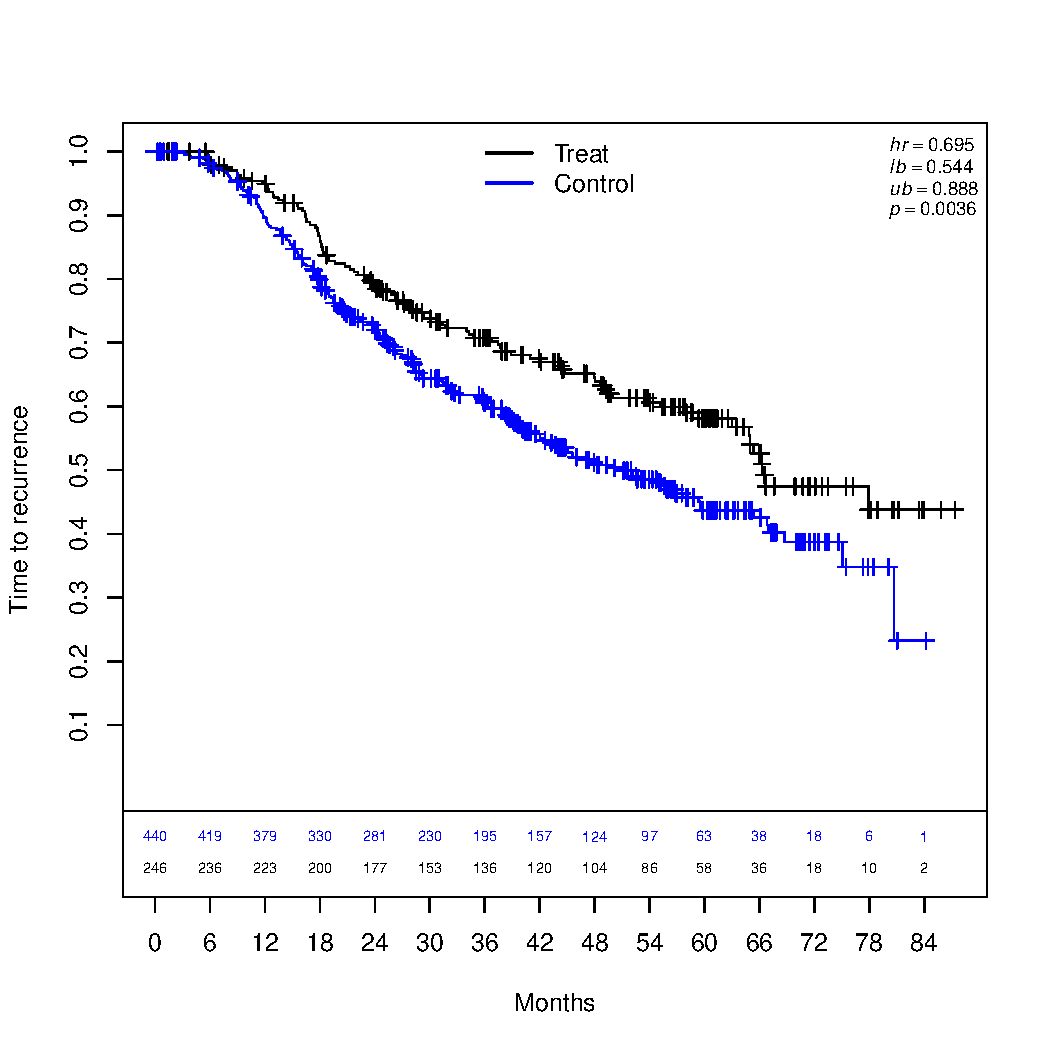
\includegraphics[width=\maxwidth]{figure/unnamed-chunk-3-1} 
\begin{kframe}\begin{verbatim}
## Super-population empirical harm and non-harm hazard ratios= NA 0.701027 
## Causal HR (empirical ITT)= 0.701027
\end{verbatim}
\begin{alltt}
\hlcom{# Creates 'dgm' list containing}
\hlkwd{print}\hlstd{(}\hlkwd{names}\hlstd{(this.dgm}\hlopt{$}\hlstd{dgm))}
\end{alltt}
\begin{verbatim}
##  [1] "df.super_rand" "sigC"          "hr.H.true"     "hr.Hc.true"   
##  [5] "cens.type"     "mu"            "hr.causal"     "b.true"       
##  [9] "sig"           "muC"           "covs.analysis" "fs.harm.true" 
## [13] "vt.harm.true"  "grf.harm.true" "model"
\end{verbatim}
\begin{alltt}
\hlcom{# df.super_rand is the 'super population' of N=5000}
\hlkwd{print}\hlstd{(}\hlkwd{names}\hlstd{(this.dgm}\hlopt{$}\hlstd{dgm}\hlopt{$}\hlstd{df.super_rand))}
\end{alltt}
\begin{verbatim}
##  [1] "pid"           "age"           "meno"          "size"         
##  [5] "grade"         "nodes"         "pgr"           "er"           
##  [9] "hormon"        "rfstime"       "status"        "v7"           
## [13] "v6"            "v5"            "v4"            "v3"           
## [17] "v2"            "v1"            "flag.harm"     "zh"           
## [21] "z5"            "z3"            "z4"            "z2"           
## [25] "z1"            "treat"         "event"         "id"           
## [29] "y"             "hlin.conf.1"   "hlin.conf.0"   "lin1.conf"    
## [33] "lin0.conf"     "lin.conf.true" "Ts"            "es"           
## [37] "h0.potential"  "h1.potential"  "linC0.conf"    "linC1.conf"   
## [41] "hlin.ratio"
\end{verbatim}
\begin{alltt}
\hlcom{# The original covariates and outcomes are returned ('super populaton'}
\hlcom{# versions) h0.potential is the subjects' potential hazard for Control per}
\hlcom{# Weibull model h1.potential is the subjects' potential hazard for Treatment}
\hlcom{# per Weibull model}

\hlcom{# The underlying marginal hazard ratio (average across potentials) for H is}
\hlkwd{print}\hlstd{(this.dgm}\hlopt{$}\hlstd{dgm}\hlopt{$}\hlstd{hr.H.true)}
\end{alltt}
\begin{verbatim}
## [1] NA
\end{verbatim}
\begin{alltt}
\hlcom{# Here it is NA since this is the null of NO subgroup So the complement and ITT}
\hlcom{# are the same}
\hlkwd{print}\hlstd{(this.dgm}\hlopt{$}\hlstd{dgm}\hlopt{$}\hlstd{hr.Hc.true)}
\end{alltt}
\begin{verbatim}
##    treat 
## 0.701027
\end{verbatim}
\begin{alltt}
\hlcom{# The ITT is 'hr.causal'}
\hlkwd{print}\hlstd{(this.dgm}\hlopt{$}\hlstd{dgm}\hlopt{$}\hlstd{hr.causal)}
\end{alltt}
\begin{verbatim}
##    treat 
## 0.701027
\end{verbatim}
\begin{alltt}
\hlcom{# Now, in the simulations for GRF we output the identification of the H}
\hlcom{# subgroup (and thus complement) that aligns with the implementation of GRF}
\hlcom{# This is 'grf.harm.true'}
\hlkwd{print}\hlstd{(this.dgm}\hlopt{$}\hlstd{dgm}\hlopt{$}\hlstd{grf.harm.true)}
\end{alltt}
\begin{verbatim}
## NULL
\end{verbatim}
\begin{alltt}
\hlcom{# Is NULL here since under the null model (No subgroup)}

\hlcom{########################## For subgroup generation}

\hlcom{# hrh.target is the desired (marginal) hazard ratio for the subgroup}
\hlstd{hrH.target} \hlkwb{<-} \hlnum{2.5}
\hlstd{mod.harm} \hlkwb{<-} \hlstr{"alt"}

\hlstd{this.dgm} \hlkwb{<-} \hlkwd{get.dgm4}\hlstd{(}\hlkwc{mod.harm} \hlstd{= mod.harm,} \hlkwc{N} \hlstd{= N,} \hlkwc{k.treat} \hlstd{= k.treat,} \hlkwc{model.index} \hlstd{= model.index,}
    \hlkwc{hrH.target} \hlstd{= hrH.target,} \hlkwc{cens.type} \hlstd{= cens.type,} \hlkwc{out.loc} \hlstd{= out.loc,} \hlkwc{file.index} \hlstd{= file.index,}
    \hlkwc{details} \hlstd{=} \hlnum{FALSE}\hlstd{)}

\hlcom{# The underlying marginal hazard ratio (average across potentials) for H is}
\hlkwd{print}\hlstd{(this.dgm}\hlopt{$}\hlstd{dgm}\hlopt{$}\hlstd{hr.H.true)}
\end{alltt}
\begin{verbatim}
##    treat 
## 2.499996
\end{verbatim}
\begin{alltt}
\hlcom{# The complement}
\hlkwd{print}\hlstd{(this.dgm}\hlopt{$}\hlstd{dgm}\hlopt{$}\hlstd{hr.Hc.true)}
\end{alltt}
\begin{verbatim}
##     treat 
## 0.6466405
\end{verbatim}
\begin{alltt}
\hlcom{# ITT}
\hlkwd{print}\hlstd{(this.dgm}\hlopt{$}\hlstd{dgm}\hlopt{$}\hlstd{hr.causal)}
\end{alltt}
\begin{verbatim}
##     treat 
## 0.7125876
\end{verbatim}
\begin{alltt}
\hlcom{# Subgroup identification for GRF}
\hlkwd{print}\hlstd{(this.dgm}\hlopt{$}\hlstd{dgm}\hlopt{$}\hlstd{grf.harm.true)}
\end{alltt}
\begin{verbatim}
## [1] "v1=1" "v3=1"
\end{verbatim}
\begin{alltt}
\hlcom{# NOTE that as H effects (hrH.target) varies, the ITT effect will also vary BUT}
\hlcom{# the complement effect is the same}

\hlcom{# For example, changing hrH.target to 1.0}
\hlstd{hrH.target} \hlkwb{<-} \hlnum{1}
\hlstd{mod.harm} \hlkwb{<-} \hlstr{"alt"}
\hlstd{this.dgm} \hlkwb{<-} \hlkwd{get.dgm4}\hlstd{(}\hlkwc{mod.harm} \hlstd{= mod.harm,} \hlkwc{N} \hlstd{= N,} \hlkwc{k.treat} \hlstd{= k.treat,} \hlkwc{model.index} \hlstd{= model.index,}
    \hlkwc{hrH.target} \hlstd{= hrH.target,} \hlkwc{cens.type} \hlstd{= cens.type,} \hlkwc{out.loc} \hlstd{= out.loc,} \hlkwc{file.index} \hlstd{= file.index,}
    \hlkwc{details} \hlstd{=} \hlnum{FALSE}\hlstd{)}
\hlcom{# The underlying marginal hazard ratio (average across potentials) for H is}
\hlkwd{print}\hlstd{(this.dgm}\hlopt{$}\hlstd{dgm}\hlopt{$}\hlstd{hr.H.true)}
\end{alltt}
\begin{verbatim}
##     treat 
## 0.9999989
\end{verbatim}
\begin{alltt}
\hlcom{# The complement}
\hlkwd{print}\hlstd{(this.dgm}\hlopt{$}\hlstd{dgm}\hlopt{$}\hlstd{hr.Hc.true)}
\end{alltt}
\begin{verbatim}
##     treat 
## 0.6466405
\end{verbatim}
\begin{alltt}
\hlcom{# ITT}
\hlkwd{print}\hlstd{(this.dgm}\hlopt{$}\hlstd{dgm}\hlopt{$}\hlstd{hr.causal)}
\end{alltt}
\begin{verbatim}
##     treat 
## 0.6754515
\end{verbatim}
\begin{alltt}
\hlcom{# Subgroup identification for GRF}
\hlkwd{print}\hlstd{(this.dgm}\hlopt{$}\hlstd{dgm}\hlopt{$}\hlstd{grf.harm.true)}
\end{alltt}
\begin{verbatim}
## [1] "v1=1" "v3=1"
\end{verbatim}
\begin{alltt}
\hlcom{# Changing hrH.target to 3.0}
\hlstd{hrH.target} \hlkwb{<-} \hlnum{3}
\hlstd{mod.harm} \hlkwb{<-} \hlstr{"alt"}
\hlstd{this.dgm} \hlkwb{<-} \hlkwd{get.dgm4}\hlstd{(}\hlkwc{mod.harm} \hlstd{= mod.harm,} \hlkwc{N} \hlstd{= N,} \hlkwc{k.treat} \hlstd{= k.treat,} \hlkwc{model.index} \hlstd{= model.index,}
    \hlkwc{hrH.target} \hlstd{= hrH.target,} \hlkwc{cens.type} \hlstd{= cens.type,} \hlkwc{out.loc} \hlstd{= out.loc,} \hlkwc{file.index} \hlstd{= file.index,}
    \hlkwc{details} \hlstd{=} \hlnum{FALSE}\hlstd{)}
\hlcom{# The underlying marginal hazard ratio (average across potentials) for H is}
\hlkwd{print}\hlstd{(this.dgm}\hlopt{$}\hlstd{dgm}\hlopt{$}\hlstd{hr.H.true)}
\end{alltt}
\begin{verbatim}
##    treat 
## 3.000004
\end{verbatim}
\begin{alltt}
\hlcom{# The complement}
\hlkwd{print}\hlstd{(this.dgm}\hlopt{$}\hlstd{dgm}\hlopt{$}\hlstd{hr.Hc.true)}
\end{alltt}
\begin{verbatim}
##     treat 
## 0.6466405
\end{verbatim}
\begin{alltt}
\hlcom{# ITT}
\hlkwd{print}\hlstd{(this.dgm}\hlopt{$}\hlstd{dgm}\hlopt{$}\hlstd{hr.causal)}
\end{alltt}
\begin{verbatim}
##     treat 
## 0.7169919
\end{verbatim}
\begin{alltt}
\hlcom{# Subgroup identification for GRF}
\hlkwd{print}\hlstd{(this.dgm}\hlopt{$}\hlstd{dgm}\hlopt{$}\hlstd{grf.harm.true)}
\end{alltt}
\begin{verbatim}
## [1] "v1=1" "v3=1"
\end{verbatim}
\end{kframe}
\end{knitrout}

\begin{knitrout}
\definecolor{shadecolor}{rgb}{0.969, 0.969, 0.969}\color{fgcolor}\begin{kframe}
\begin{alltt}
\hlcom{# Simulate with hrH=2.5 pH ~ 13% (12.5)}

\hlstd{hrH.target} \hlkwb{<-} \hlnum{2.5}
\hlstd{mod.harm} \hlkwb{<-} \hlstr{"alt"}

\hlstd{this.dgm} \hlkwb{<-} \hlkwd{get.dgm4}\hlstd{(}\hlkwc{mod.harm} \hlstd{= mod.harm,} \hlkwc{N} \hlstd{= N,} \hlkwc{k.treat} \hlstd{= k.treat,} \hlkwc{model.index} \hlstd{= model.index,}
    \hlkwc{hrH.target} \hlstd{= hrH.target,} \hlkwc{cens.type} \hlstd{= cens.type,} \hlkwc{out.loc} \hlstd{= out.loc,} \hlkwc{file.index} \hlstd{= file.index,}
    \hlkwc{details} \hlstd{=} \hlnum{TRUE}\hlstd{)}
\end{alltt}
\end{kframe}
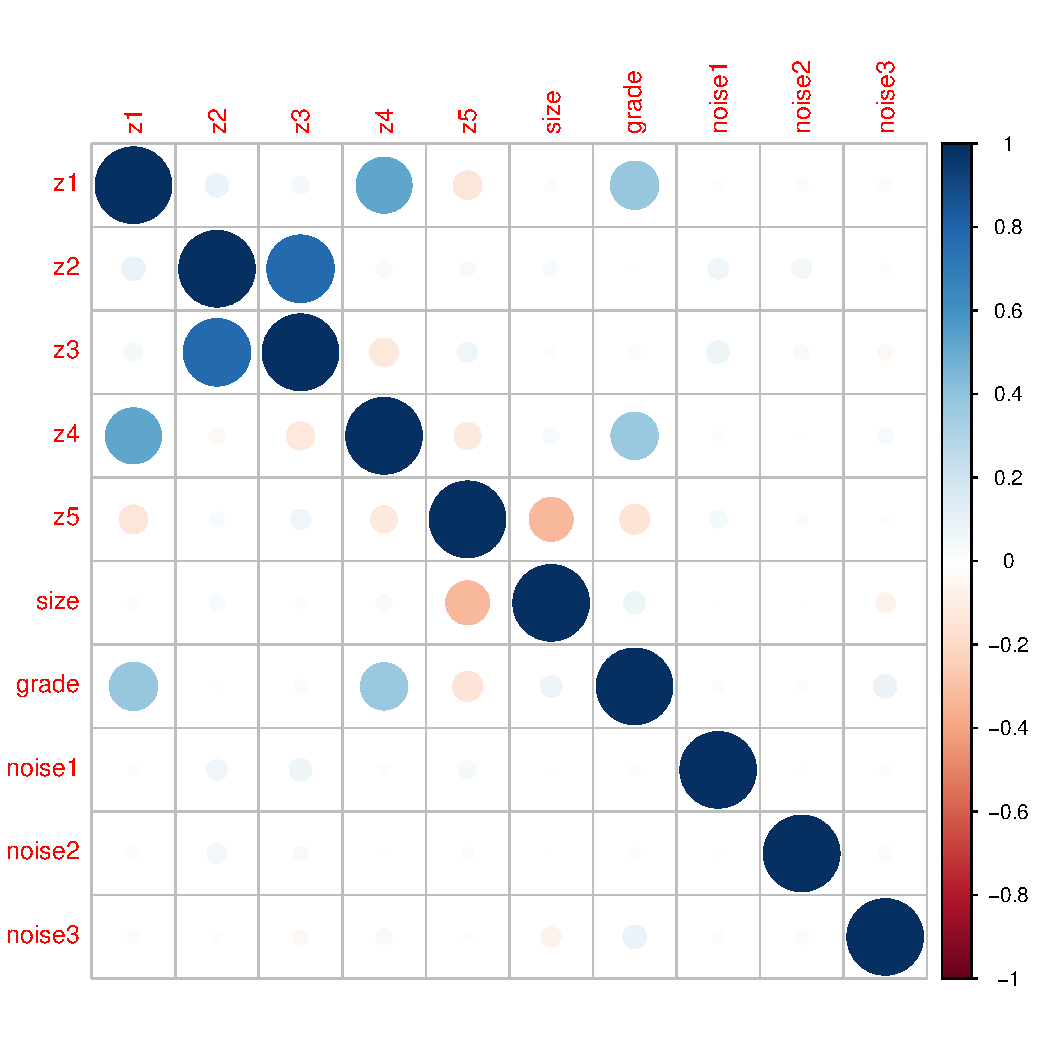
\includegraphics[width=\maxwidth]{figure/unnamed-chunk-4-1} 
\begin{kframe}\begin{verbatim}
## Super-population empirical harm and non-harm hazard ratios= 2.499996 0.6466405 
## Causal HR (empirical ITT)= 0.7125876
\end{verbatim}
\begin{alltt}
\hlcom{# The underlying marginal hazard ratio (average across potentials) for H is}
\hlkwd{print}\hlstd{(this.dgm}\hlopt{$}\hlstd{dgm}\hlopt{$}\hlstd{hr.H.true)}
\end{alltt}
\begin{verbatim}
##    treat 
## 2.499996
\end{verbatim}
\begin{alltt}
\hlcom{# The complement}
\hlkwd{print}\hlstd{(this.dgm}\hlopt{$}\hlstd{dgm}\hlopt{$}\hlstd{hr.Hc.true)}
\end{alltt}
\begin{verbatim}
##     treat 
## 0.6466405
\end{verbatim}
\begin{alltt}
\hlcom{# ITT}
\hlkwd{print}\hlstd{(this.dgm}\hlopt{$}\hlstd{dgm}\hlopt{$}\hlstd{hr.causal)}
\end{alltt}
\begin{verbatim}
##     treat 
## 0.7125876
\end{verbatim}
\begin{alltt}
\hlcom{# Subgroup identification for GRF}
\hlkwd{print}\hlstd{(this.dgm}\hlopt{$}\hlstd{dgm}\hlopt{$}\hlstd{grf.harm.true)}
\end{alltt}
\begin{verbatim}
## [1] "v1=1" "v3=1"
\end{verbatim}
\begin{alltt}
\hlcom{# The data-generating model for the sims is dgm}

\hlstd{dgm} \hlkwb{<-} \hlstd{this.dgm}\hlopt{$}\hlstd{dgm}
\hlcom{# The covariates for the analysis}
\hlstd{confounders.name} \hlkwb{<-} \hlstd{dgm}\hlopt{$}\hlstd{covs.analysis}
\hlkwd{print}\hlstd{(confounders.name)}
\end{alltt}
\begin{verbatim}
## [1] "v1" "v2" "v3" "v4" "v5" "v6" "v7"
\end{verbatim}
\begin{alltt}
\hlcom{# Note that the true model is the first 5 The last 2 are 'noise' covariates}

\hlcom{# Randomly chose a simulation seed (based on the simulation number=sim) Note:}
\hlcom{# sim<-1 returns NO estimated subgroup}
\hlstd{sim} \hlkwb{<-} \hlnum{5}
\hlstd{x} \hlkwb{<-} \hlkwd{sim_aftm4_gbsg}\hlstd{(}\hlkwc{dgm} \hlstd{= dgm,} \hlkwc{n} \hlstd{= N,} \hlkwc{maxFollow} \hlstd{= maxFollow,} \hlkwc{muC.adj} \hlstd{= muC.adj,} \hlkwc{simid} \hlstd{= sim,}
    \hlkwc{drawtreat} \hlstd{=} \hlnum{TRUE}\hlstd{)}

\hlcom{# KM curves for simulated data}
\hlkwd{plot_onesample}\hlstd{(}\hlkwc{df} \hlstd{= x,} \hlkwc{tte.name} \hlstd{=} \hlstr{"y.sim"}\hlstd{,} \hlkwc{event.name} \hlstd{=} \hlstr{"event.sim"}\hlstd{,} \hlkwc{treat.name} \hlstd{=} \hlstr{"treat"}\hlstd{,}
    \hlkwc{fix.rows} \hlstd{=} \hlnum{FALSE}\hlstd{,} \hlkwc{byrisk} \hlstd{=} \hlnum{6}\hlstd{,} \hlkwc{show.med} \hlstd{=} \hlnum{TRUE}\hlstd{)}
\end{alltt}
\end{kframe}
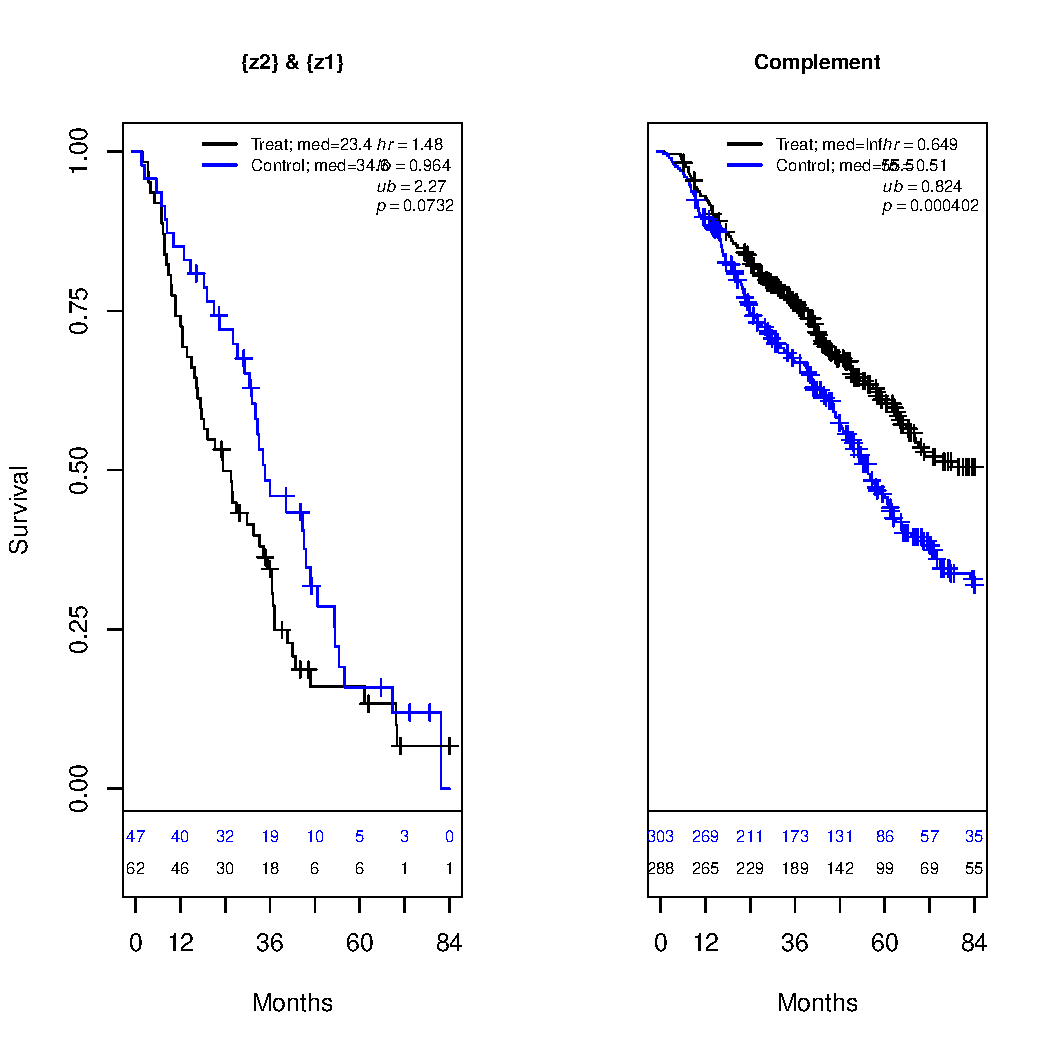
\includegraphics[width=\maxwidth]{figure/unnamed-chunk-4-2} 
\begin{kframe}\begin{alltt}
\hlcom{# Returns simulated data (event.sim,y.sim) with covariates from the observed}
\hlcom{# data flag.harm indicates whether the subject is in the H subgroup}
\hlkwd{print}\hlstd{(}\hlkwd{table}\hlstd{(x}\hlopt{$}\hlstd{flag.harm))}
\end{alltt}
\begin{verbatim}
## 
##   0   1 
## 608  92
\end{verbatim}
\begin{alltt}
\hlcom{# The covariates and subgroups are random}

\hlcom{# prop H summaries (%'s and sizes)}
\hlstd{sizeH_true} \hlkwb{<-} \hlkwd{with}\hlstd{(x,} \hlkwd{sum}\hlstd{(flag.harm))}
\hlstd{propH_true} \hlkwb{<-} \hlkwd{with}\hlstd{(x,} \hlkwd{mean}\hlstd{(flag.harm))}
\hlstd{sizeHc_true} \hlkwb{<-} \hlkwd{with}\hlstd{(x,} \hlkwd{sum}\hlstd{(}\hlopt{!}\hlstd{flag.harm))}
\hlstd{propHc_true} \hlkwb{<-} \hlkwd{with}\hlstd{(x,} \hlkwd{mean}\hlstd{(}\hlopt{!}\hlstd{flag.harm))}
\hlstd{dfHpop} \hlkwb{<-} \hlkwd{data.table}\hlstd{(sim, sizeH_true, propH_true, sizeHc_true, propHc_true)}

\hlkwd{print}\hlstd{(dfHpop)}
\end{alltt}
\begin{verbatim}
##    sim sizeH_true propH_true sizeHc_true propHc_true
## 1:   5         92  0.1314286         608   0.8685714
\end{verbatim}
\begin{alltt}
\hlcom{# GRF analysis with frac.tau=0.6 This uses 60% of the maximum truncation value}
\hlcom{# for RMST That is, if t1 (t0) is max event time for treatment (control) Then}
\hlcom{# RMST uses tau = 0.6*min(t0,t1)}

\hlstd{ansGRF} \hlkwb{<-} \hlkwa{NULL}
\hlstd{analysis} \hlkwb{<-} \hlstr{"GRF"}

\hlstd{showdetails} \hlkwb{<-} \hlnum{TRUE}

\hlstd{grf.est} \hlkwb{<-} \hlkwd{try}\hlstd{(}\hlkwd{grf.subg.harm.survival}\hlstd{(}\hlkwc{data} \hlstd{= x,} \hlkwc{confounders.name} \hlstd{= confounders.name,}
    \hlkwc{outcome.name} \hlstd{= outcome.name,} \hlkwc{event.name} \hlstd{= event.name,} \hlkwc{id.name} \hlstd{= id.name,} \hlkwc{treat.name} \hlstd{= treat.name,}
    \hlkwc{n.min} \hlstd{= n.min,} \hlkwc{dmin.grf} \hlstd{= dmin.grf,} \hlkwc{frac.tau} \hlstd{= frac.tau,} \hlkwc{details} \hlstd{= showdetails),}
    \hlnum{TRUE}\hlstd{)}
\end{alltt}
\begin{verbatim}
## tau= 48.87494 
##    leaf.node control.mean control.size control.se treated.mean treated.size
## 1          2    -5.839009   391.000000   1.478196     5.839009   391.000000
## 2          3     4.382296   309.000000   1.540356    -4.382296   309.000000
## 3          2    -2.979152   490.000000   1.238637     2.979152   490.000000
## 4          4   -10.003601   118.000000   2.648085    10.003601   118.000000
## 5          5    18.600939    92.000000   2.804837   -18.600939    92.000000
## 11         5   -10.003601   118.000000   2.648085    10.003601   118.000000
## 21         8    -5.819074   239.000000   1.911168     5.819074   239.000000
## 51        11    -1.450641   107.000000   2.008444     1.450641   107.000000
## 6         12    -6.929135    63.000000   3.634465     6.929135    63.000000
## 7         13    20.627202    83.000000   2.881148   -20.627202    83.000000
##    treated.se       diff depth
## 1    1.478196 -11.678019     1
## 2    1.540356   8.764592     1
## 3    1.238637  -5.958305     2
## 4    2.648085 -20.007202     2
## 5    2.804837  37.201879     2
## 11   2.648085 -20.007202     3
## 21   1.911168 -11.638149     3
## 51   2.008444  -2.901282     3
## 6    3.634465 -13.858270     3
## 7    2.881148  41.254403     3
##   leaf.node control.mean control.size control.se treated.mean treated.size
## 7        13    20.627202    83.000000   2.881148   -20.627202    83.000000
##   treated.se    diff depth
## 7   2.881148 41.2544     3
\end{verbatim}
\begin{alltt}
\hlcom{# GRF applied to trees of depths 1, 2, and 3 tree 1 is depth 1 (etc)}

\hlkwd{print}\hlstd{(}\hlkwd{names}\hlstd{(grf.est))}
\end{alltt}
\begin{verbatim}
## [1] "data"       "grf.gsub"   "sg.harm.id" "harm.any"   "tree"      
## [6] "tau.rmst"   "tree1"      "tree2"      "tree3"
\end{verbatim}
\begin{alltt}
\hlcom{# 'tree' corresponds to the selected H subgroup}

\hlcom{# Plotting does not work in knitr But these will show the forest trees}

\hlcom{# plot(grf.est$tree1) plot(grf.est$tree2) plot(grf.est$tree3)}

\hlcom{# The tree corresponding to selected subgroup plot(grf.est$tree)}

\hlcom{# If a subgroup is selected (meets GRF criteria) then the subgroup id is output}
\hlkwd{print}\hlstd{(grf.est}\hlopt{$}\hlstd{sg.harm.id)}
\end{alltt}
\begin{verbatim}
## [1] "v1=2" "v2=2" "v3=2" "v4=2"
\end{verbatim}
\begin{alltt}
\hlcom{# If NO subgroup then sg.harm.id will be NULL}

\hlcom{# Any subgroups with (causal) treatment effects in favor of control are stored}
\hlcom{# here}
\hlkwd{print}\hlstd{(grf.est}\hlopt{$}\hlstd{harm.any)}
\end{alltt}
\begin{verbatim}
##   leaf.node control.mean control.size control.se treated.mean treated.size
## 2         3     4.382296   309.000000   1.540356    -4.382296   309.000000
## 5         5    18.600939    92.000000   2.804837   -18.600939    92.000000
## 7        13    20.627202    83.000000   2.881148   -20.627202    83.000000
##   treated.se      diff depth
## 2   1.540356  8.764592     1
## 5   2.804837 37.201879     2
## 7   2.881148 41.254403     3
\end{verbatim}
\begin{alltt}
\hlcom{# Next, output Cox model estimates}

\hlkwa{if} \hlstd{(}\hlopt{!}\hlkwd{inherits}\hlstd{(grf.est,} \hlstr{"try-error"}\hlstd{)) \{}

    \hlstd{ansGRF} \hlkwb{<-} \hlkwd{grf.estimates.out}\hlstd{(}\hlkwc{df} \hlstd{= x,} \hlkwc{grf.est} \hlstd{= grf.est,} \hlkwc{dgm} \hlstd{= dgm,} \hlkwc{cox.formula.sim} \hlstd{= cox.formula.sim,}
        \hlkwc{cox.formula.adj.sim} \hlstd{= cox.formula.adj.sim,} \hlkwc{analysis} \hlstd{= analysis,} \hlkwc{frac.tau} \hlstd{= frac.tau)}

    \hlstd{ansGRF} \hlkwb{<-} \hlkwd{cbind}\hlstd{(dfHpop, ansGRF)}

    \hlkwd{print}\hlstd{(}\hlkwd{names}\hlstd{(ansGRF))}

    \hlcom{# Plot the estimated subgroup}

    \hlcom{# Note: grf.est$data is the analysis dataset with the GRF subgroup flag}
    \hlcom{# attached 'treat.recommend=0' is the estimated H subgroup}
    \hlcom{# 'treat.recommend=1' is the estimated H^c subgroup}

    \hlstd{df0.grf} \hlkwb{<-} \hlkwd{subset}\hlstd{(grf.est}\hlopt{$}\hlstd{data, treat.recommend} \hlopt{==} \hlnum{0}\hlstd{)}
    \hlstd{df1.grf} \hlkwb{<-} \hlkwd{subset}\hlstd{(grf.est}\hlopt{$}\hlstd{data, treat.recommend} \hlopt{==} \hlnum{1}\hlstd{)}

    \hlkwd{par}\hlstd{(}\hlkwc{mfrow} \hlstd{=} \hlkwd{c}\hlstd{(}\hlnum{1}\hlstd{,} \hlnum{2}\hlstd{))}
    \hlkwd{plot.subgroup}\hlstd{(}\hlkwc{sub1} \hlstd{= df0.grf,} \hlkwc{sub1C} \hlstd{= df1.grf,} \hlkwc{tte.name} \hlstd{=} \hlstr{"y.sim"}\hlstd{,} \hlkwc{event.name} \hlstd{=} \hlstr{"event.sim"}\hlstd{,}
        \hlkwc{treat.name} \hlstd{=} \hlstr{"treat"}\hlstd{,} \hlkwc{fix.rows} \hlstd{=} \hlnum{FALSE}\hlstd{,} \hlkwc{byrisk} \hlstd{=} \hlnum{9}\hlstd{,} \hlkwc{legend.cex} \hlstd{=} \hlnum{0.6}\hlstd{,} \hlkwc{show.med} \hlstd{=} \hlnum{FALSE}\hlstd{,}
        \hlkwc{subid} \hlstd{=} \hlkwd{deparse}\hlstd{(grf.est}\hlopt{$}\hlstd{sg.harm.id))}

    \hlcom{# NOTE that the classification metrics naming is not standard npv is the %}
    \hlcom{# of the estimated H^c (est(H^c), say) that are correctly classified}
    \hlcom{# specificity is the % of the H^c population represented by est(H^c) ppv is}
    \hlcom{# the % of the estimated H (est(H), say) that are correctly classified}
    \hlcom{# sensitivity is the % of the H population represented by est(H)}

    \hlcom{# The true size and 'estimated size' (size of estimated subgroup)}
    \hlkwd{print}\hlstd{(ansGRF[,} \hlkwd{c}\hlstd{(}\hlstr{"sizeH_true"}\hlstd{,} \hlstr{"size.H"}\hlstd{)])}

    \hlcom{# Complement}
    \hlkwd{print}\hlstd{(ansGRF[,} \hlkwd{c}\hlstd{(}\hlstr{"sizeHc_true"}\hlstd{,} \hlstr{"size.Hc"}\hlstd{)])}

    \hlcom{# Classification summaries}
    \hlkwd{print}\hlstd{(ansGRF[,} \hlkwd{c}\hlstd{(}\hlstr{"npv"}\hlstd{,} \hlstr{"specificity"}\hlstd{,} \hlstr{"ppv"}\hlstd{,} \hlstr{"sensitivity"}\hlstd{)])}

    \hlcom{# The Cox estimates and CIs for estimated subgroups These are all}
    \hlcom{# un-adjusted (raw) H true (est,lower,upper)}
    \hlkwd{print}\hlstd{(ansGRF[,} \hlkwd{c}\hlstd{(}\hlstr{"hr.H.true"}\hlstd{,} \hlstr{"l.H.true"}\hlstd{,} \hlstr{"u.H.true"}\hlstd{)])}
    \hlcom{# GRF H estimate (est,lower,upper)}
    \hlkwd{print}\hlstd{(ansGRF[,} \hlkwd{c}\hlstd{(}\hlstr{"hr.H.hat"}\hlstd{,} \hlstr{"l.H.hat"}\hlstd{,} \hlstr{"u.H.hat"}\hlstd{)])}
    \hlcom{# Complement H^c true (est,lower,upper)}
    \hlkwd{print}\hlstd{(ansGRF[,} \hlkwd{c}\hlstd{(}\hlstr{"hr.Hc.true"}\hlstd{,} \hlstr{"l.Hc.true"}\hlstd{,} \hlstr{"u.Hc.true"}\hlstd{)])}
    \hlcom{# GRF H^c estimate (est,lower,upper)}
    \hlkwd{print}\hlstd{(ansGRF[,} \hlkwd{c}\hlstd{(}\hlstr{"hr.Hc.hat"}\hlstd{,} \hlstr{"l.Hc.hat"}\hlstd{,} \hlstr{"u.Hc.hat"}\hlstd{)])}

    \hlcom{# ITT}
    \hlkwd{print}\hlstd{(ansGRF[,} \hlkwd{c}\hlstd{(}\hlstr{"hr.itt"}\hlstd{,} \hlstr{"l.itt"}\hlstd{,} \hlstr{"u.itt"}\hlstd{)])}
\hlstd{\}}
\end{alltt}
\begin{verbatim}
##  [1] "sim"         "sizeH_true"  "propH_true"  "sizeHc_true" "propHc_true"
##  [6] "any.H"       "size.H"      "size.Hc"     "ppv"         "npv"        
## [11] "specificity" "sensitivity" "found.1"     "found.2"     "found.both" 
## [16] "found.al3"   "hr.H.true"   "hr.Hc.true"  "hr.H.hat"    "hr.Hc.hat"  
## [21] "b1.H"        "b2.H"        "b1.Hc"       "b2.Hc"       "p.cens"     
## [26] "analysis"    "taumax"      "hr.itt"      "l.itt"       "u.itt"      
## [31] "hr.adj.itt"  "l.adj.itt"   "u.adj.itt"   "l.H.true"    "u.H.true"   
## [36] "l.Hc.true"   "u.Hc.true"   "l.H.hat"     "u.H.hat"     "l.Hc.hat"   
## [41] "u.Hc.hat"
\end{verbatim}
\end{kframe}
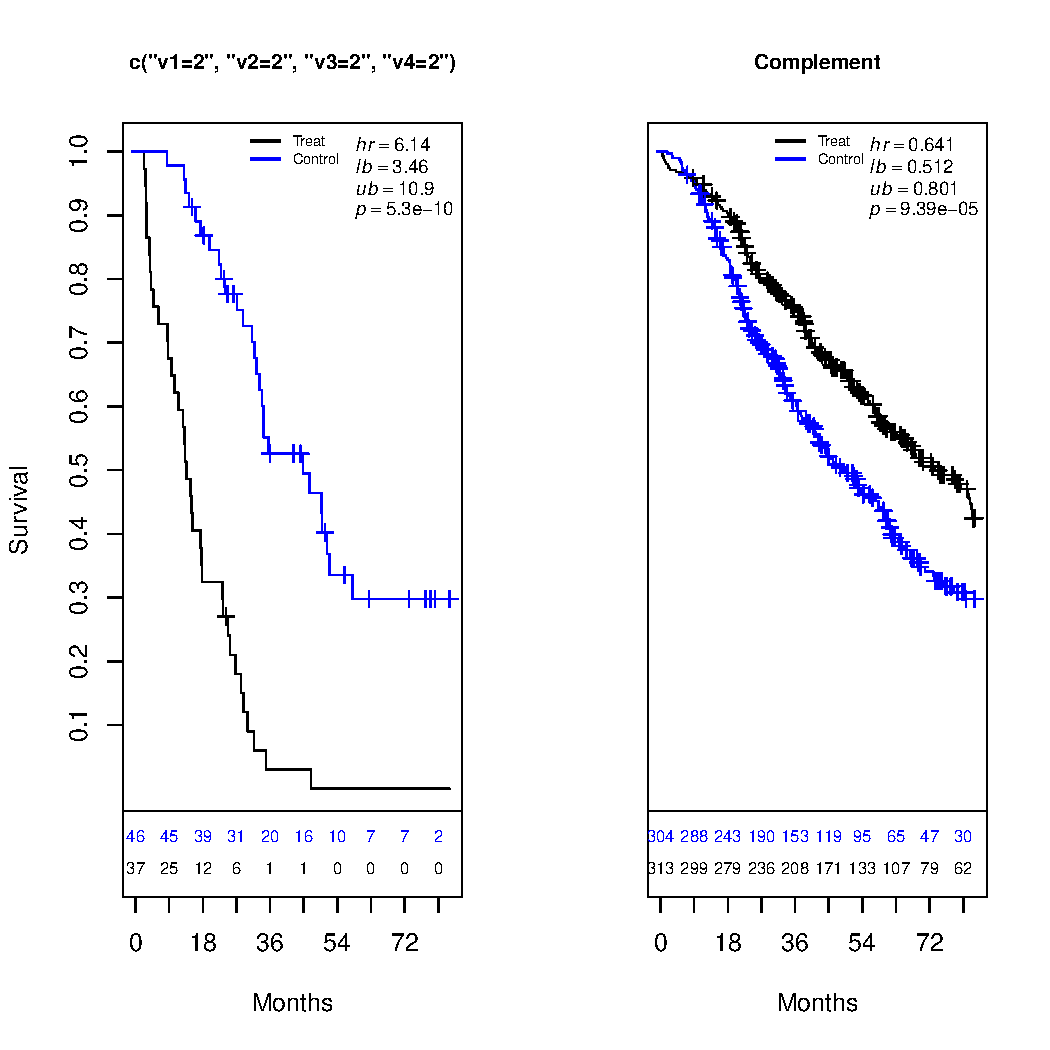
\includegraphics[width=\maxwidth]{figure/unnamed-chunk-4-3} 
\begin{kframe}\begin{verbatim}
##    sizeH_true size.H
## 1:         92     83
##    sizeHc_true size.Hc
## 1:         608     617
##    npv specificity       ppv sensitivity
## 1:   1   0.9854133 0.9021739           1
##    hr.H.true l.H.true u.H.true
## 1:   4.75023 2.841556 7.940962
##    hr.H.hat  l.H.hat  u.H.hat
## 1: 6.136099 3.461193 10.87825
##    hr.Hc.true l.Hc.true u.Hc.true
## 1:  0.6259481  0.499205   0.78487
##    hr.Hc.hat  l.Hc.hat  u.Hc.hat
## 1: 0.6407118 0.5124452 0.8010839
##       hr.itt     l.itt     u.itt
## 1: 0.7819166 0.6382393 0.9579379
\end{verbatim}
\begin{alltt}
\hlcom{# If GRF is not 'estimable' then consider NO subgroup found Consider grf.est =}
\hlcom{# NULL}
\hlkwa{if} \hlstd{(}\hlkwd{inherits}\hlstd{(grf.est,} \hlstr{"try-error"}\hlstd{)) \{}
    \hlstd{ansGRF} \hlkwb{<-} \hlkwd{grf.estimates.out}\hlstd{(}\hlkwc{df} \hlstd{= x,} \hlkwc{grf.est} \hlstd{=} \hlkwa{NULL}\hlstd{,} \hlkwc{dgm} \hlstd{= dgm,} \hlkwc{cox.formula.sim} \hlstd{= cox.formula.sim,}
        \hlkwc{cox.formula.adj.sim} \hlstd{= cox.formula.adj.sim,} \hlkwc{analysis} \hlstd{= analysis,} \hlkwc{frac.tau} \hlstd{=} \hlnum{1}\hlstd{)}
    \hlstd{ansGRF} \hlkwb{<-} \hlkwd{cbind}\hlstd{(dfHpop, ansGRF)}
    \hlkwa{if} \hlstd{(}\hlkwd{round}\hlstd{(}\hlkwd{c}\hlstd{(ansGRF}\hlopt{$}\hlstd{hr.Hc.hat} \hlopt{-} \hlstd{ansGRF}\hlopt{$}\hlstd{hr.itt),} \hlnum{6}\hlstd{)} \hlopt{!=} \hlnum{0}\hlstd{)}
        \hlkwd{stop}\hlstd{(}\hlstr{"Cox hr for H-complement NOT equal to ITT (GRF)"}\hlstd{)}
\hlstd{\}}
\end{alltt}
\end{kframe}
\end{knitrout}
\bibliographystyle{spbasic}      % basic style, author-year citations
\bibliography{../../subgroups_ref}
\end{document}
